\documentclass[12pt]{article}
\usepackage{graphicx}
\usepackage{epstopdf} %converting to PDF
\begin{document}

\title{DCM III: Homework}
\author{Kevin Aquino}
\maketitle

\section{Homework set}
For this homework we will get to understand parts of the Balloon model as well as keep up our skills in understanding dynamic equations.
\subsection{Set I}
For the first set, we will get to solve the Flow equations which are given by the following:
\begin{eqnarray}
\frac{ds}{dt} =& z(t) - \kappa s - \gamma(f-1), \\
\frac{df}{dt} =& s,
\end{eqnarray}
with the conditions at $t=0$, $f=1$, $s=0$, and setting the input $z(t)$ as:
\begin{equation}
z(t) = 0.5\exp\left[-(t-2)^2/0.1\right].
\end{equation}
Initially use the following numbers for the parameters: $\kappa=0.65$ and $\gamma=0.41$. Remember to use what we have learned spefiically that:
\begin{equation}
\frac{ds}{dt} \approx \frac{\Delta s}{\Delta t} = \frac{s_{t_{i+1}} -  s_{t_{i}}}{\Delta t}.
\end{equation}
And use this approximation for $f$ as well. For the numerical simulation set $\Delta t = 0.001$, and set the maximum length of $t$ to be $50$ You should have the following solution in Figure 1.Make sure you get the figures right before moving on!. 
\begin{figure}[h!]
\centering
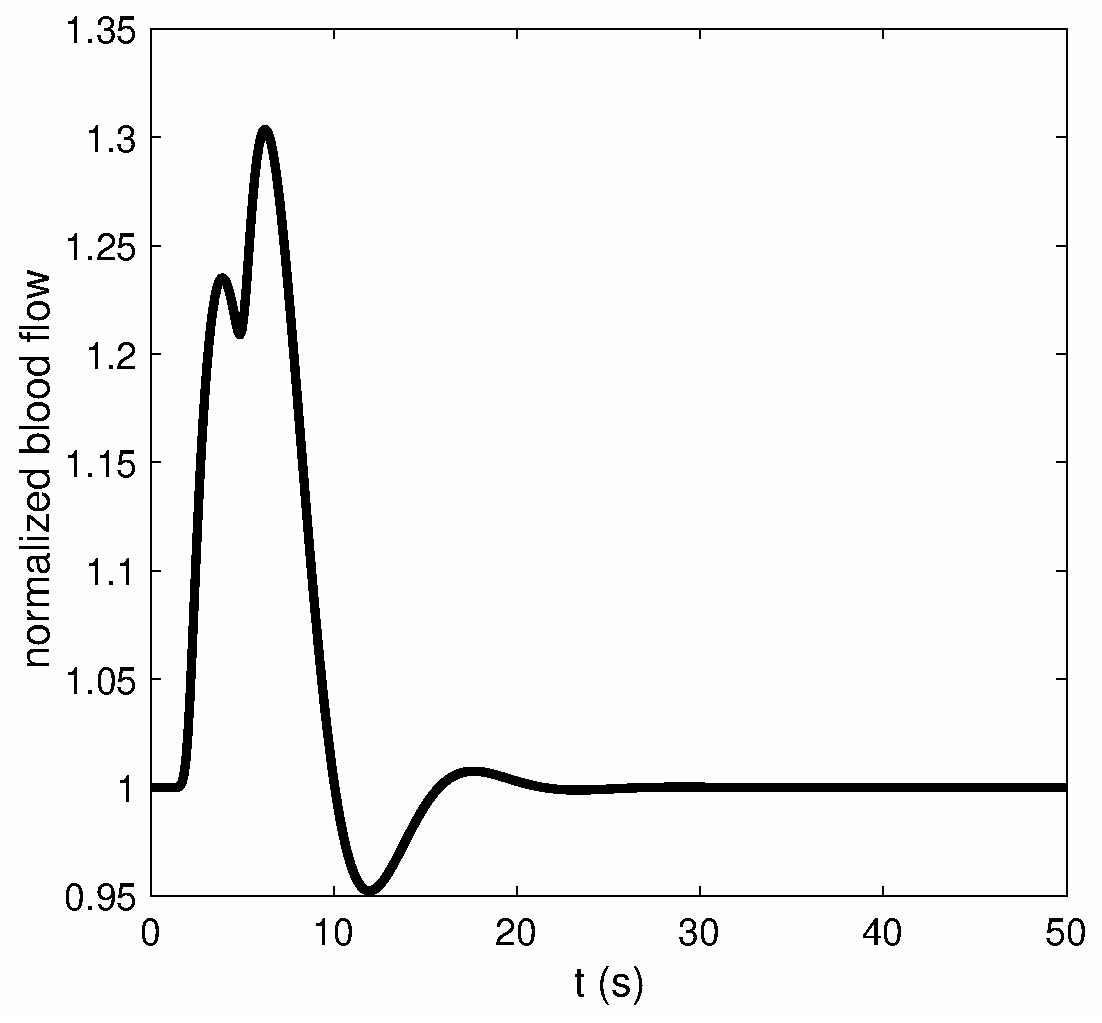
\includegraphics[width=0.5\linewidth]{flow.eps}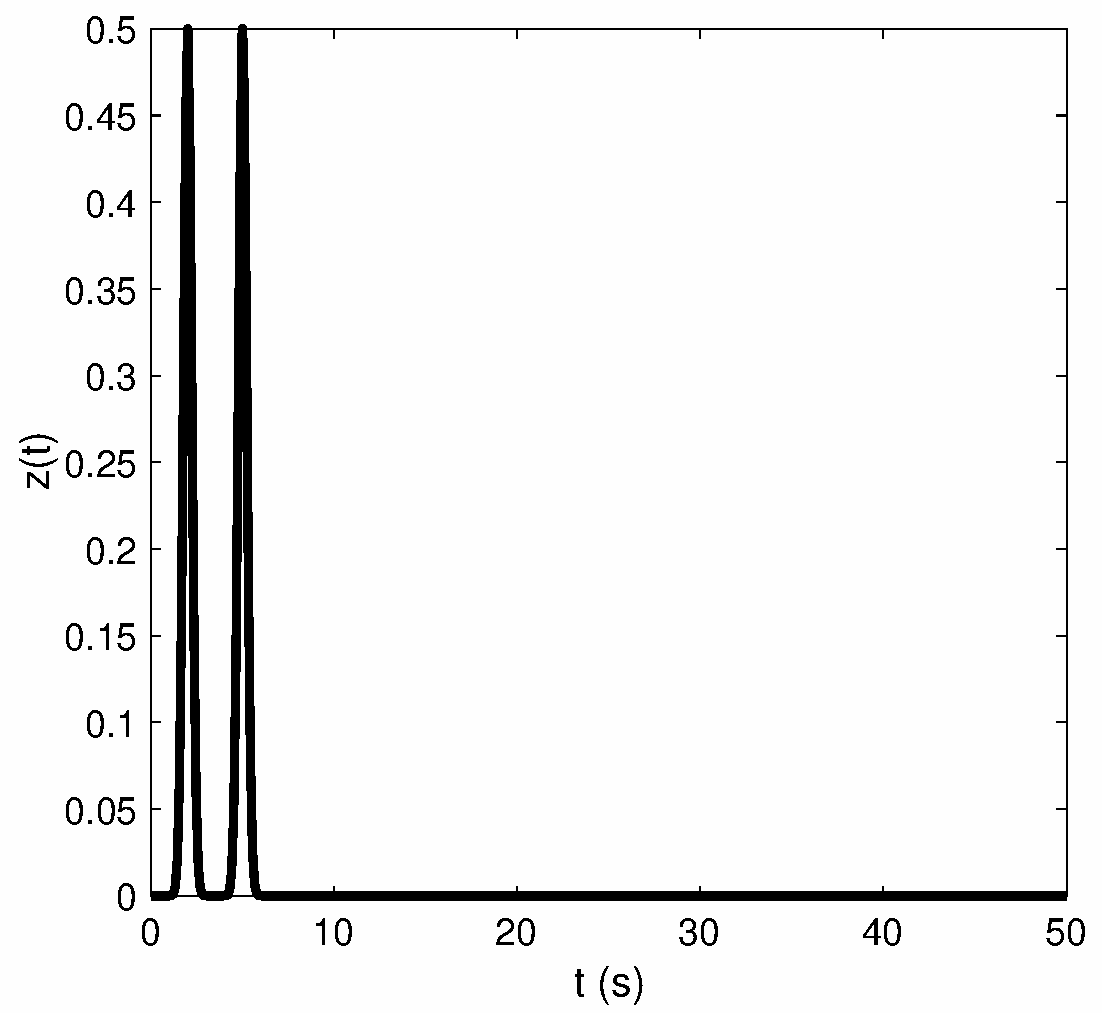
\includegraphics[width=0.5\linewidth]{input.eps}
\caption{What the solution should look like}
\end{figure}

\subsection{Set II}
After you have completed Set I, then simulate the same system using:
\begin{equation}
z(t) = 0.5\exp\left[-(t-2)^2/0.1\right] + 0.5\exp\left[-(t-\tau)^2/0.1\right]  .
\end{equation}
where $\tau$ is $3$. After this plot the flow response for $\tau=4,5,6,7$. Have a look at the responses and save/print out for next session!.
\subsection{Set III}
Finally repeat what we did in Set I, changing $\kappa=0.3,0.7$ and then keep $\kappa$ constant and set $\gamma = 0.2,0.8$. 

Have all these plots ready in some electronic or printed format! :) 
\end{document}
